\documentclass{beamer}

% UTF-8
\usepackage[utf8]{inputenc}
\usepackage[T1]{fontenc}

% Unnumbered appendix slides
\usepackage{appendixnumberbeamer}

% Fancy beamer theme
\usetheme{metropolis}

% Better hyphenation etc.
\usepackage{microtype}

% Graphics & Plots
\usepackage{graphicx}

% Subfigures
\usepackage{subcaption}

% SI units
\usepackage{siunitx}

% HMM drawings etc.
\usepackage{tikz}
\usetikzlibrary{arrows.meta}
\tikzset{>=Triangle[]}

\title{Gesture Recognition with a Neuromorphic Vision Sensor and Deep Learning}
\author{Marten Lienen}
\date{}

\begin{document}

\maketitle

\begin{frame}{Image vs. Event Histogram}
  \begin{figure}
    \centering
    \begin{subfigure}{0.4\textwidth}
      \centering
      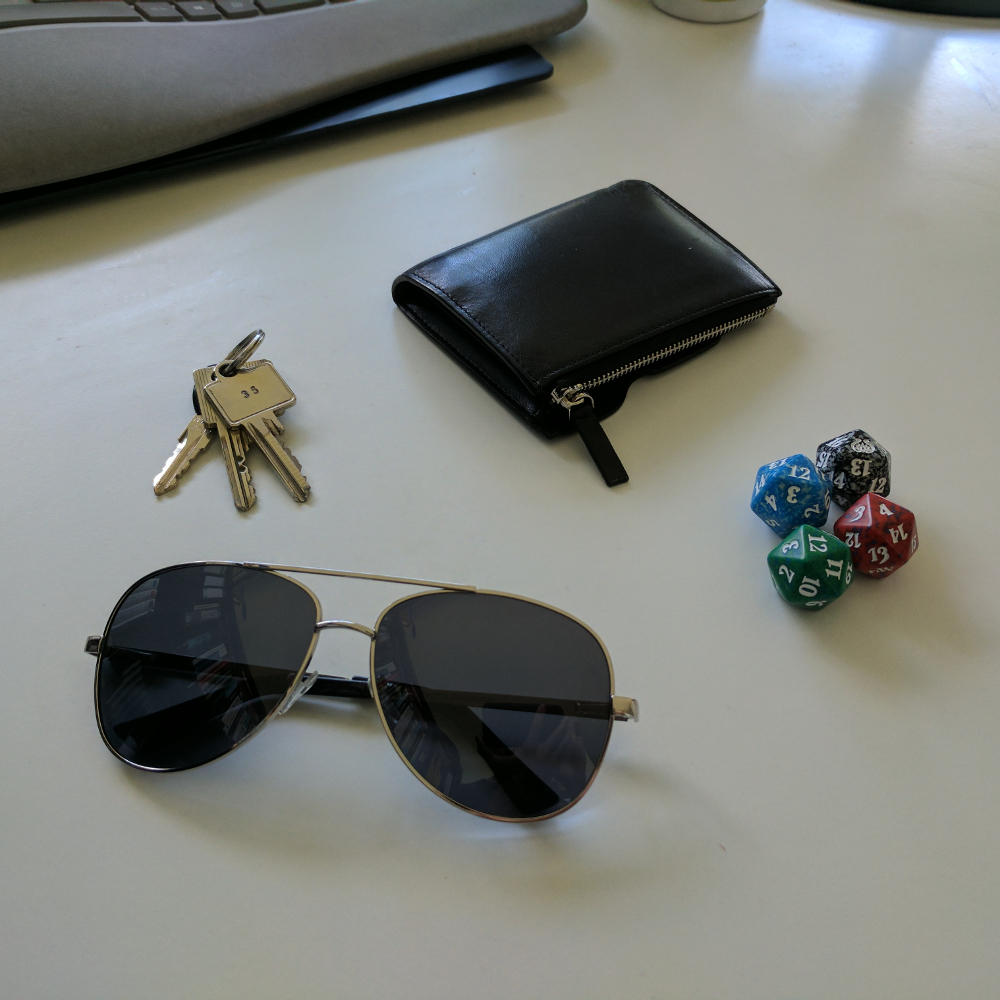
\includegraphics[width=\textwidth]{figures/objects-camera}
    \end{subfigure}
    \hspace{0.35in}
    \begin{subfigure}{0.4\textwidth}
      \centering
      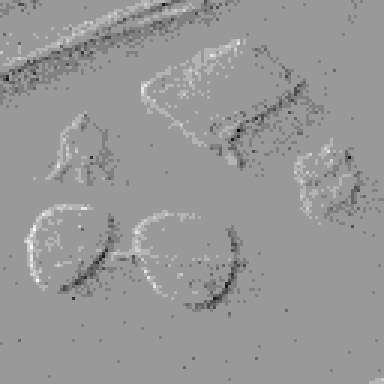
\includegraphics[width=\textwidth]{figures/objects-dvs}
    \end{subfigure}
  \end{figure}
\end{frame}

\begin{frame}{The Event Stream}
  \makebox[\textwidth][c]{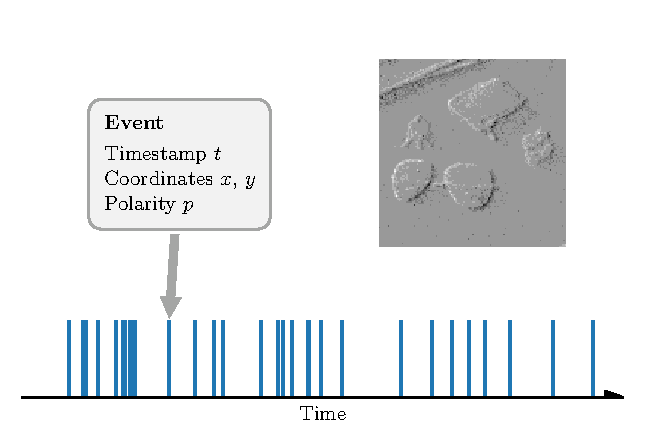
\includegraphics{figures/event-stream}}
\end{frame}

\begin{frame}{Dataset}
  \begin{itemize}
  \item 16 gestures
  \item 2 subjects
  \item 40 segmented recordings
  \item 40 minutes and 640 examples in total
  \end{itemize}
\end{frame}

\begin{frame}{Preprocessing}
  \begin{itemize}
  \item Translation invariance in time $\Delta t_{i} \leftarrow t_{i} - t_{i - 1}$
  \item Translation invariance in space
    \begin{itemize}
    \item Means with exponentially decaying weights as point of reference
    \item Halflife of \SI{50}{\milli\second} and \SI{1}{\second}
    \end{itemize}
  \item Feature Normalization
  \end{itemize}
\end{frame}

\begin{frame}{Neural Networks}
  \begin{figure}
    \centering
    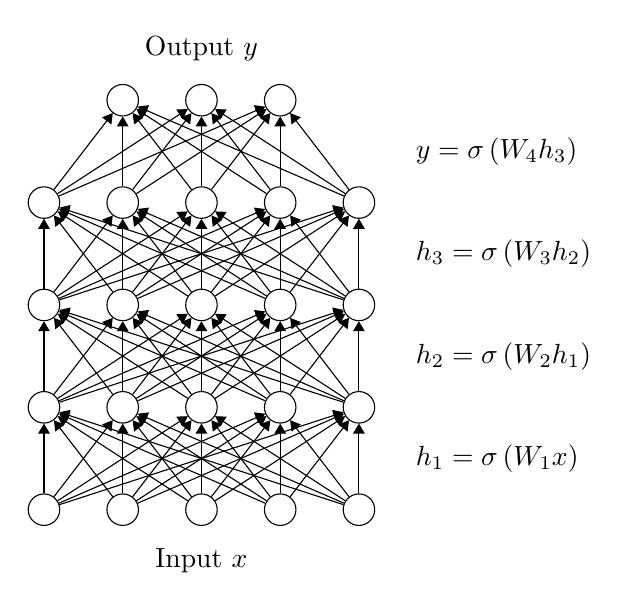
\begin{tikzpicture}[yscale=1.3]
      \node[align=center] at (3, -0.5) {Input $x$};
      \node[align=center] at (3, 4.5) {Output $y$};

      \node[anchor=west] at (5.6, 0.5) {$h_{1} = \sigma\left( W_{1}x \right)$};
      \node[anchor=west] at (5.6, 1.5) {$h_{2} = \sigma\left( W_{2}h_{1} \right)$};
      \node[anchor=west] at (5.6, 2.5) {$h_{3} = \sigma\left( W_{3}h_{2} \right)$};
      \node[anchor=west] at (5.6, 3.5) {$y = \sigma\left( W_{4}h_{3} \right)$};

      \foreach \t in {1, 2, 3, 4, 5} {
        \node[draw,circle,minimum size=0.4cm](1\t) at (\t, 0) {~};
      }

      \foreach \t in {1, 2, 3, 4, 5} {
        \node[draw,circle,minimum size=0.4cm](2\t) at (\t, 1) {~};

        \foreach \s in {1, 2, 3, 4, 5} {
          \draw[->] (1\s) -- (2\t);
        }
      }

      \foreach \t in {1, 2, 3, 4, 5} {
        \node[draw,circle,minimum size=0.4cm](3\t) at (\t, 2) {~};

        \foreach \s in {1, 2, 3, 4, 5} {
          \draw[->] (2\s) -- (3\t);
        }
      }

      \foreach \t in {1, 2, 3, 4, 5} {
        \node[draw,circle,minimum size=0.4cm](4\t) at (\t, 3) {~};

        \foreach \s in {1, 2, 3, 4, 5} {
          \draw[->] (3\s) -- (4\t);
        }
      }

      \foreach \t in {2, 3, 4} {
        \node[draw,circle,minimum size=0.4cm](5\t) at (\t, 4) {~};

        \foreach \s in {1, 2, 3, 4, 5} {
          \draw[->] (4\s) -- (5\t);
        }
      }
    \end{tikzpicture}
  \end{figure}
\end{frame}

\begin{frame}{Autoencoders}
  \begin{figure}
    \centering
    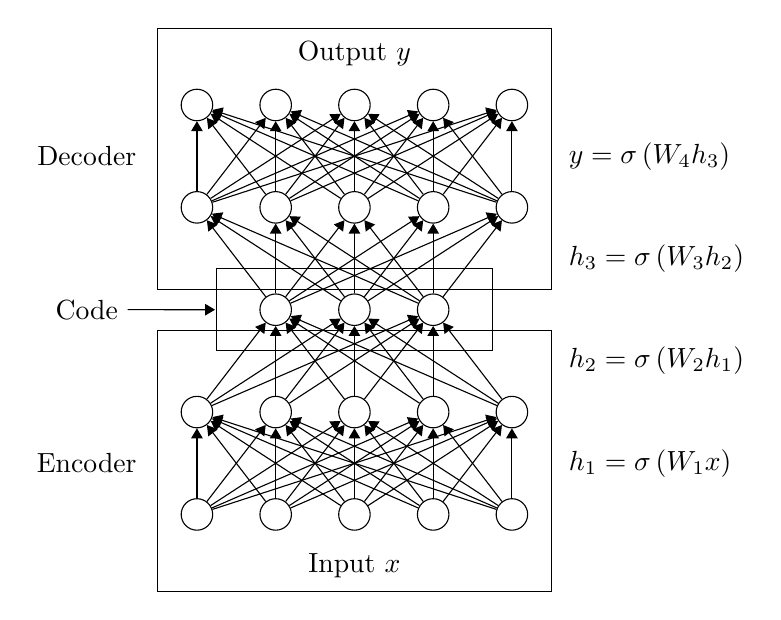
\begin{tikzpicture}[yscale=1.3]
      \node[align=center] at (3, -0.5) {Input $x$};
      \node[align=center] at (3, 4.5) {Output $y$};

      \node[align=center](code) at (-0.4, 2) {Code};
      \draw (1.25, 1.6) rectangle (4.75, 2.4);
      \draw[->] (code) -- (1.23, 2);

      \node[align=center] at (-0.4, 0.5) {Encoder};
      \draw (0.5, -0.75) rectangle (5.5, 1.8);

      \node[align=center] at (-0.4, 3.5) {Decoder};
      \draw (0.5, 2.2) rectangle (5.5, 4.75);

      \node[anchor=west] at (5.6, 0.5) {$h_{1} = \sigma\left( W_{1}x \right)$};
      \node[anchor=west] at (5.6, 1.5) {$h_{2} = \sigma\left( W_{2}h_{1} \right)$};
      \node[anchor=west] at (5.6, 2.5) {$h_{3} = \sigma\left( W_{3}h_{2} \right)$};
      \node[anchor=west] at (5.6, 3.5) {$y = \sigma\left( W_{4}h_{3} \right)$};

      \foreach \t in {1, 2, 3, 4, 5} {
        \node[draw,circle,minimum size=0.4cm](1\t) at (\t, 0) {~};
      }

      \foreach \t in {1, 2, 3, 4, 5} {
        \node[draw,circle,minimum size=0.4cm](2\t) at (\t, 1) {~};

        \foreach \s in {1, 2, 3, 4, 5} {
          \draw[->] (1\s) -- (2\t);
        }
      }

      \foreach \t in {2, 3, 4} {
        \node[draw,circle,minimum size=0.4cm](3\t) at (\t, 2) {~};

        \foreach \s in {1, 2, 3, 4, 5} {
          \draw[->] (2\s) -- (3\t);
        }
      }

      \foreach \t in {1, 2, 3, 4, 5} {
        \node[draw,circle,minimum size=0.4cm](4\t) at (\t, 3) {~};

        \foreach \s in {2, 3, 4} {
          \draw[->] (3\s) -- (4\t);
        }
      }

      \foreach \t in {1, 2, 3, 4, 5} {
        \node[draw,circle,minimum size=0.4cm](5\t) at (\t, 4) {~};

        \foreach \s in {1, 2, 3, 4, 5} {
          \draw[->] (4\s) -- (5\t);
        }
      }
    \end{tikzpicture}
  \end{figure}
\end{frame}

\begin{frame}{Recurrent Neural Networks}
  \begin{figure}
    \centering
    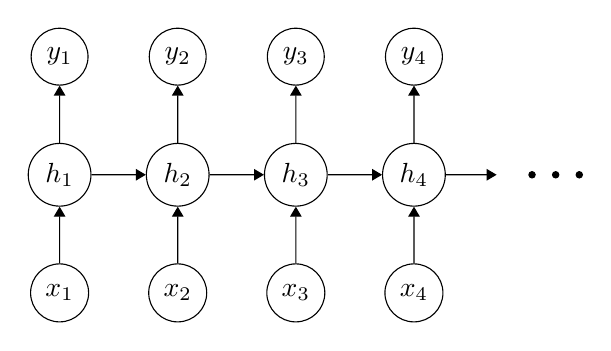
\begin{tikzpicture}[scale=1.5]
      \foreach \t in {1, 2, 3, 4} {
        \node[draw,circle](x\t) at (\t, 0) {$x_{\t}$};
        \node[draw,circle](h\t) at (\t, 1) {$h_{\t}$};
        \node[draw,circle](y\t) at (\t, 2) {$y_{\t}$};

        \draw[->] (x\t) -- (h\t);
        \draw[->] (h\t) -- (y\t);
      }

      \foreach \t [evaluate=\t as \tnext using int(\t + 1)] in {1, 2, 3} {
        \draw[->] (h\t) -- (h\tnext);
      }

      \draw[->] (h4) -- (4.7,1);
      \foreach \p [evaluate=\p as \x using (5 + 1/5 * \p)] in {0, 1, 2} {
        \fill (\x, 1) node[draw,circle,fill,inner sep=0,minimum size=0.08cm]{};
      }
    \end{tikzpicture}
  \end{figure}
  \begin{equation*}
    h_{t} = \sigma\left( Wx_{t} + Uh_{t - 1} \right)
  \end{equation*}
\end{frame}

\begin{frame}{Recurrent Autoencoders}
  \begin{figure}
    \centering
    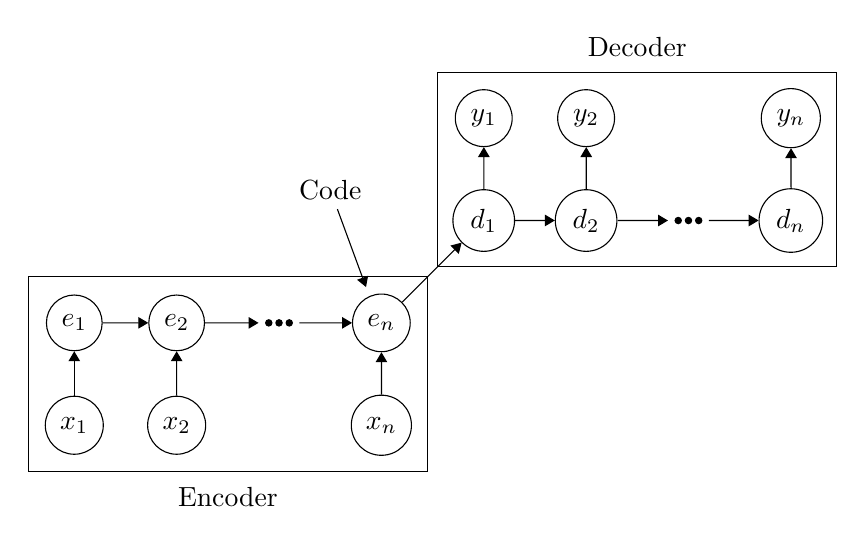
\begin{tikzpicture}[scale=1.3]
      \node[draw,circle](x1) at (0, 0) {$x_{1}$};
      \node[draw,circle](x2) at (1, 0) {$x_{2}$};
      \node[draw,circle](xn) at (3, 0) {$x_{n}$};
      \node[draw,circle](e1) at (0, 1) {$e_{1}$};
      \node[draw,circle](e2) at (1, 1) {$e_{2}$};
      \node[draw,circle](en) at (3, 1) {$e_{n}$};

      \node[align=center](code) at (2.5, 2.3) {Code};
      \draw[->] (code) -- (2.85, 1.35);

      \node[align=center] at (1.5, -0.7) {Encoder};
      \draw (-0.45, -0.45) rectangle (3.45, 1.45);

      \node[align=center] at (5.5, 3.7) {Decoder};
      \draw (3.55, 1.55) rectangle (7.45, 3.45);

      \fill (1.9, 1) node[draw,circle,fill,inner sep=0,minimum size=0.08cm]{};
      \fill (2.0, 1) node[draw,circle,fill,inner sep=0,minimum size=0.08cm]{};
      \fill (2.1, 1) node[draw,circle,fill,inner sep=0,minimum size=0.08cm]{};

      \draw[->] (x1) -- (e1);
      \draw[->] (x2) -- (e2);
      \draw[->] (xn) -- (en);

      \draw[->] (e1) -- (e2);
      \draw[->] (e2) -- (1.8, 1);
      \draw[->] (2.2, 1) -- (en);

      \node[draw,circle](y1) at (4, 3) {$y_{1}$};
      \node[draw,circle](y2) at (5, 3) {$y_{2}$};
      \node[draw,circle](yn) at (7, 3) {$y_{n}$};
      \node[draw,circle](d1) at (4, 2) {$d_{1}$};
      \node[draw,circle](d2) at (5, 2) {$d_{2}$};
      \node[draw,circle](dn) at (7, 2) {$d_{n}$};

      \fill (5.9, 2) node[draw,circle,fill,inner sep=0,minimum size=0.08cm]{};
      \fill (6.0, 2) node[draw,circle,fill,inner sep=0,minimum size=0.08cm]{};
      \fill (6.1, 2) node[draw,circle,fill,inner sep=0,minimum size=0.08cm]{};

      \draw[->] (d1) -- (y1);
      \draw[->] (d2) -- (y2);
      \draw[->] (dn) -- (yn);

      \draw[->] (d1) -- (d2);
      \draw[->] (d2) -- (5.8, 2);
      \draw[->] (6.2, 2) -- (dn);

      \draw[->] (en) -- (d1);
    \end{tikzpicture}
  \end{figure}
\end{frame}

\begin{frame}{Event Sequence Compression}
  \makebox[\textwidth][c]{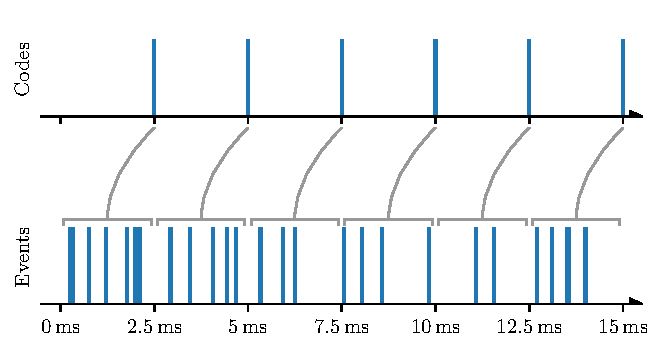
\includegraphics{figures/autoencoder}}
\end{frame}

\begin{frame}{Learned Representations}
  \begin{figure}
    \centering
    \begin{subfigure}{0.49\textwidth}
      \centering
      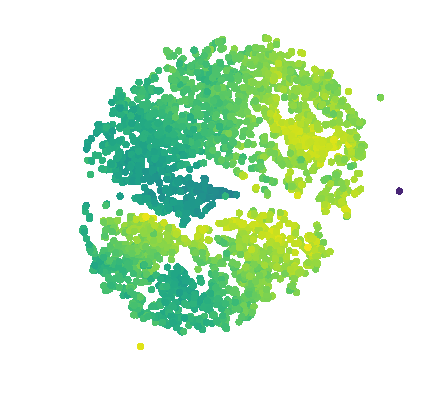
\includegraphics[width=\textwidth]{figures/push-hand-up}
      \caption{Push Hand Up}
    \end{subfigure}
    \begin{subfigure}{0.49\textwidth}
      \centering
      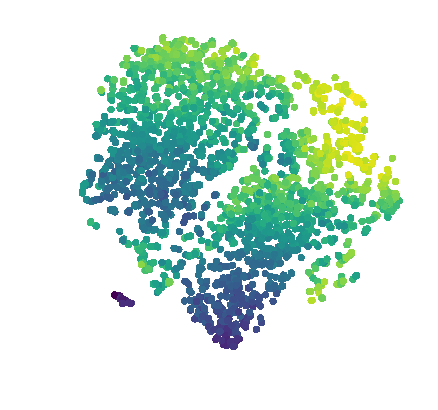
\includegraphics[width=\textwidth]{figures/swipe-right}
      \caption{Swipe Right}
    \end{subfigure}
  \end{figure}
\end{frame}

\begin{frame}{Framewise Classification}
  % early stopping
  \begin{figure}
    \centering
    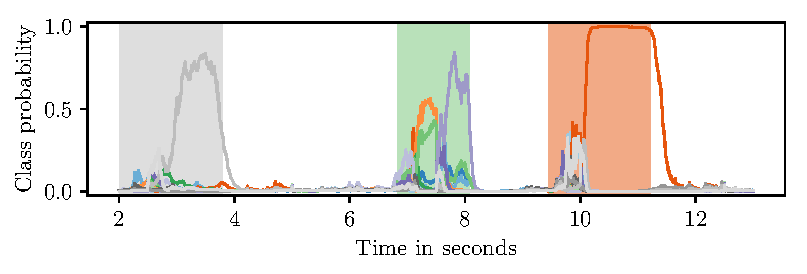
\includegraphics[width=\textwidth]{figures/framewise-output}
  \end{figure}
\end{frame}

\begin{frame}{HMM Decoding}
  \begin{figure}
    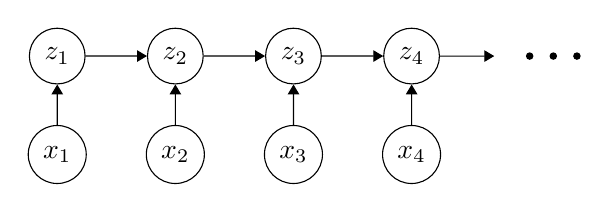
\begin{tikzpicture}[xscale=1.5,yscale=1.25]
      \foreach \t in {1, 2, 3, 4} {
        \node[draw,circle](x\t) at (\t, 0) {$x_{\t}$};
        \node[draw,circle](z\t) at (\t, 1) {$z_{\t}$};

        \draw[->] (x\t) -- (z\t);
      }

      \foreach \t [evaluate=\t as \tnext using int(\t + 1)] in {1, 2, 3} {
        \draw[->] (z\t) -- (z\tnext);
      }

      \draw[->] (z4) -- (4.7,1);
      \foreach \p [evaluate=\p as \x using (5 + 1/5 * \p)] in {0, 1, 2} {
        \fill (\x, 1) node[draw,circle,fill,inner sep=0,minimum size=0.08cm]{};
      }
    \end{tikzpicture}
  \end{figure}
  \begin{figure}
    \centering
    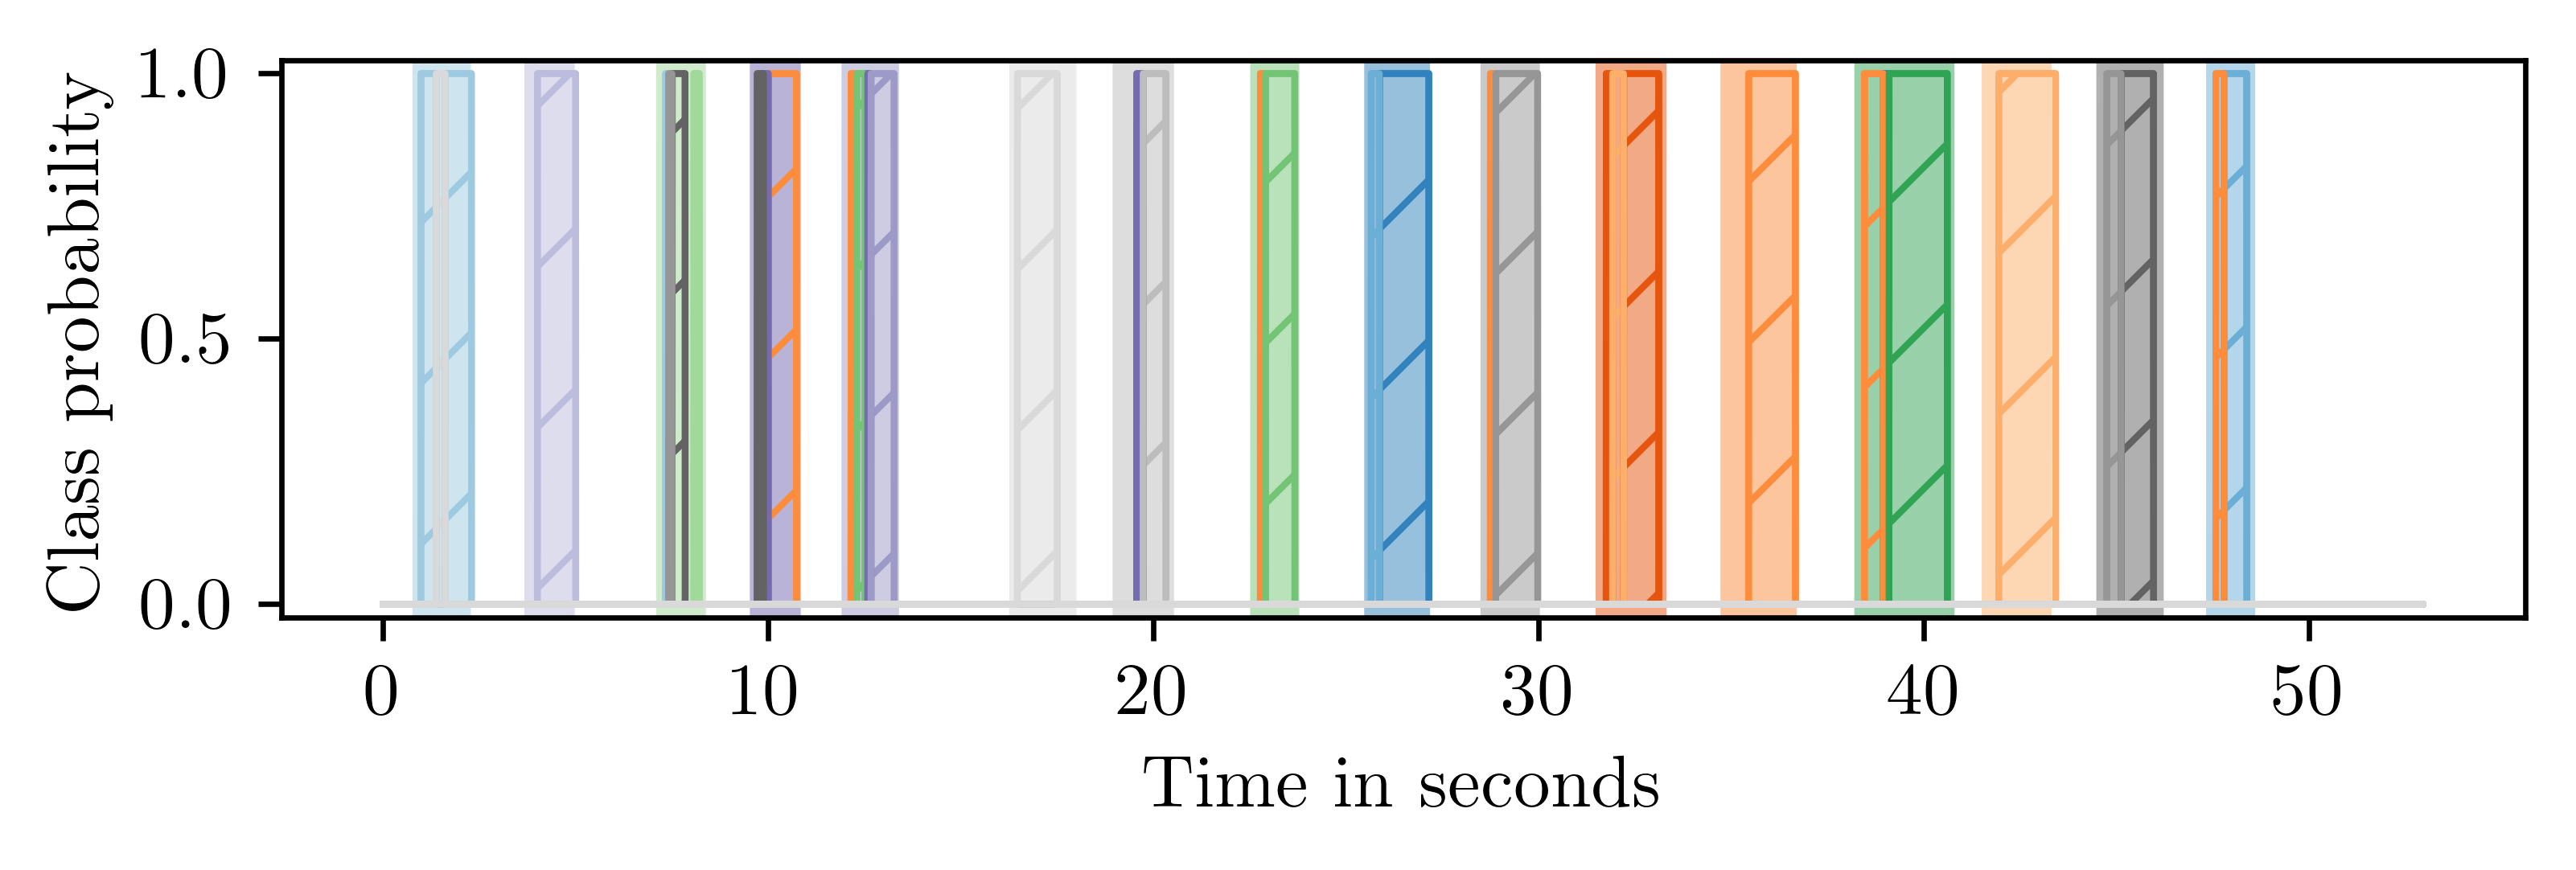
\includegraphics[width=\textwidth]{figures/decoded}
  \end{figure}
\end{frame}

\begin{frame}{HMM Segmentation}
  \begin{figure}
    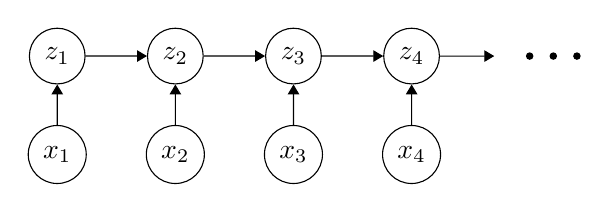
\begin{tikzpicture}[xscale=1.5,yscale=1.25]
      \foreach \t in {1, 2, 3, 4} {
        \node[draw,circle](x\t) at (\t, 0) {$x_{\t}$};
        \node[draw,circle](z\t) at (\t, 1) {$z_{\t}$};

        \draw[->] (x\t) -- (z\t);
      }

      \foreach \t [evaluate=\t as \tnext using int(\t + 1)] in {1, 2, 3} {
        \draw[->] (z\t) -- (z\tnext);
      }

      \draw[->] (z4) -- (4.7,1);
      \foreach \p [evaluate=\p as \x using (5 + 1/5 * \p)] in {0, 1, 2} {
        \fill (\x, 1) node[draw,circle,fill,inner sep=0,minimum size=0.08cm]{};
      }
    \end{tikzpicture}
  \end{figure}
  \begin{figure}
    \centering
    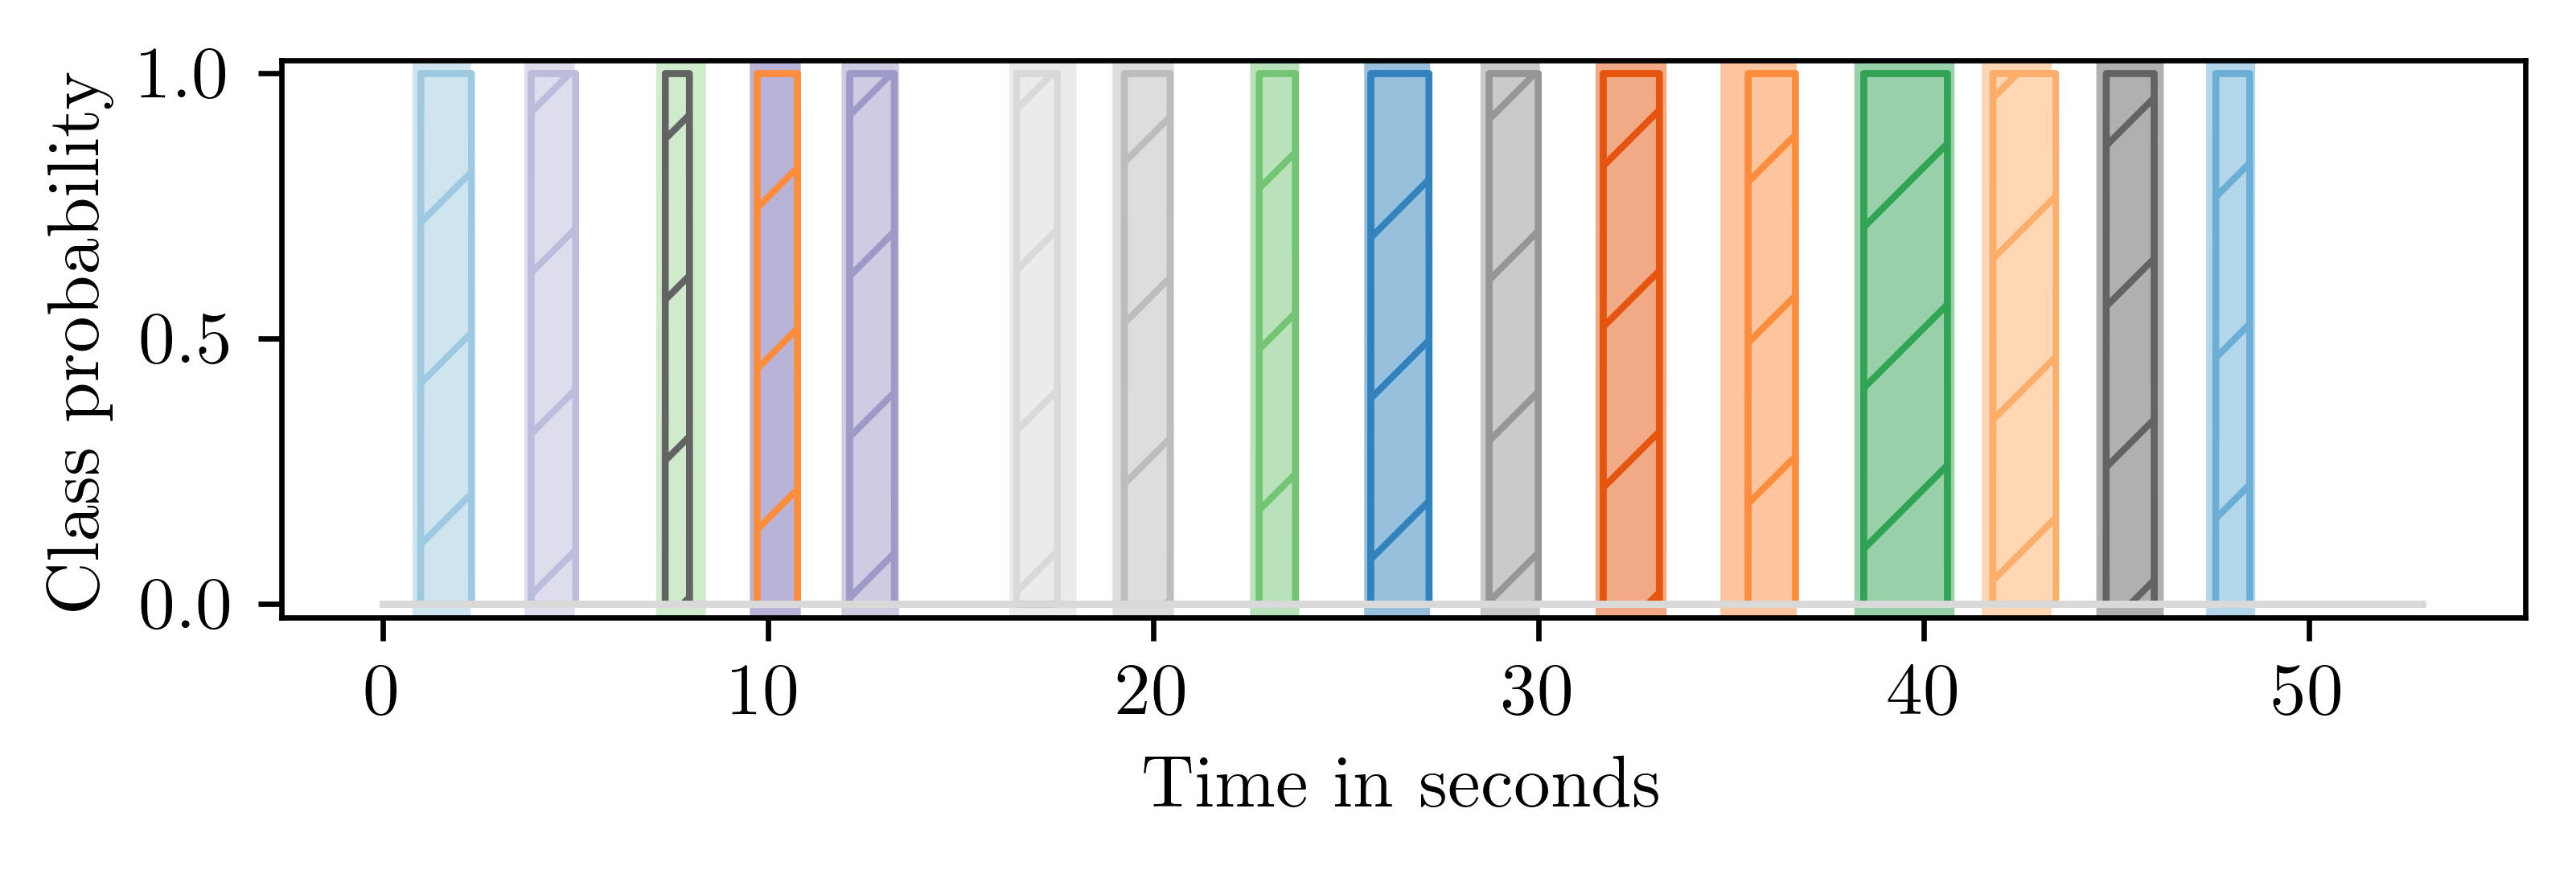
\includegraphics[width=\textwidth]{figures/segmented}
  \end{figure}
\end{frame}

\begin{frame}{Predictions}
  \begin{figure}
    \centering
    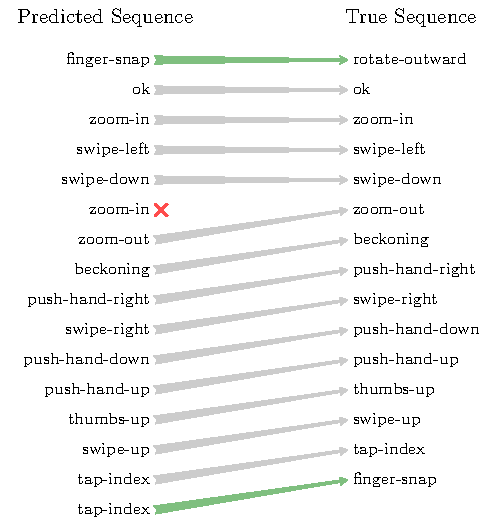
\includegraphics[height=3in]{figures/levenshtein}
  \end{figure}
\end{frame}

\begin{frame}{Results}
  \begin{figure}[h]
    \centering
    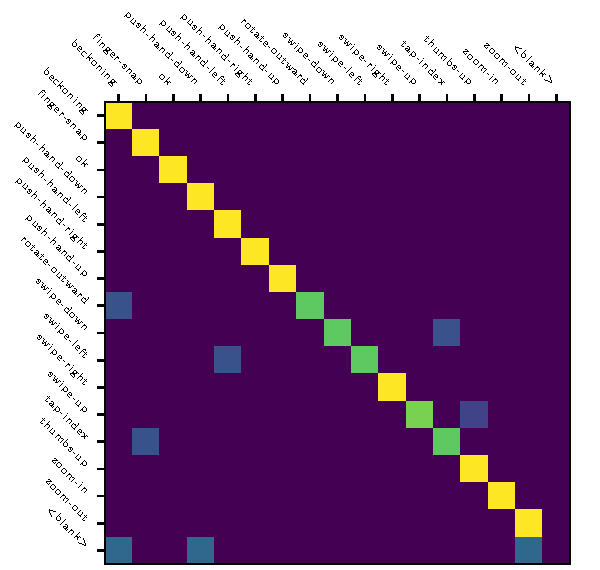
\includegraphics[height=2.5in]{figures/confusion-matrix}
  \end{figure}
  Mean Levenshtein Distance 2.0, Label Error Rate 0.125
\end{frame}

\begin{frame}[standout]{}
  Thank You
\end{frame}

\appendix

\begin{frame}{Methods}
  \vspace{0.2in}
  \makebox[\textwidth][c]{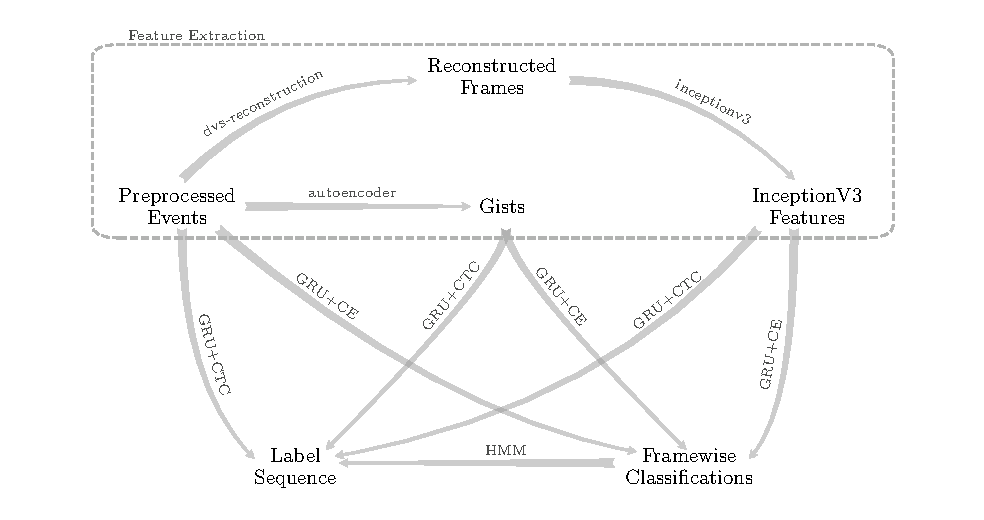
\includegraphics[width=5.5in]{figures/methods}}
\end{frame}

\begin{frame}{Frame Reconstructions}
  \begin{figure}
    \centering
    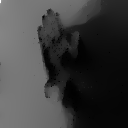
\includegraphics[width=3cm]{figures/reconstructed-1}
    \hspace{0.7cm}
    
\includegraphics[width=3cm]{figures/reconstructed-2}
    \hspace{0.7cm}
    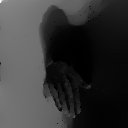
\includegraphics[width=3cm]{figures/reconstructed-3}
  \end{figure}
\end{frame}

\end{document}
